\documentclass[11pt]{article}
\usepackage{graphicx}
\graphicspath{ {images/} }
\usepackage{url}
\usepackage{epigraph}
\usepackage{float}
\usepackage{wrapfig}
\usepackage{listings}
\usepackage{multirow}
\usepackage{hyperref}
\usepackage{amsfonts}
\usepackage{amsmath}
\usepackage{array}
\usepackage{etoolbox}
\usepackage{yax}
\usepackage{hyperref}
\usepackage{dutch}
\selectlanguage{dutch}


\setparameter Cantrell:
 firstname   = Colin
 lastname    = Cantrell
 title       = {Architect}
 email       = {\href{mailto:colin@nexus.io}{colin@nexus.io}}

\setparameter Gmyrek:
 firstname   = Bryan
 lastname    = "Gmyrek Ph.D."
 title       = {Developer}
 email       = {\href{mailto:bryan@nexus.io}{bryan@nexus.io}}
 
\setparameter Reeg:
 firstname   = Kierre
 lastname    = Reeg
 title       = {Visionary}
 email       = {\href{mailto:kierre@nexus.io}{kierre@nexus.io}}
 
\setparameter pSmith:
 firstname   = Preston
 lastname    = Smith
 title       = {Community Manager}
 email       = {\href{mailto:preston@nexus.io}{preston@nexus.io}}
 
 \setparameter kSmith:
 firstname   = Keith
 lastname    = Smith
 title       = {Cryptocurrency Expert}
 email       = {\href{mailto:keith@nexus.io}{keith@nexus.io}}
 
  \setparameter jSmith:
 firstname   = Jacynda
 lastname    = Smith
 title       = {Cryptocurrency Expert}
 email       = {\href{mailto:jacynda@nexus.io}{jacynda@nexus.io}}
 
 \setparameter Mara:
 firstname   = Mara
 lastname    = Michael
 title       = {Editor}
 email       = {\href{mailto:maramichael@q.com}{maramichael@q.com}}
 
 \setparameter gBogaerts:
 firstname   = Glenn
 lastname    = Bogaerts
 title       = {Vertaler}
 email       = {\href{mailto:glenn@bossit.be}{glenn@bossit.be}}
 
 \setparameter Nexus:
 firstname   = {Geschreven door sommigen van ons,}
 lastname    = {Gegeven door ons allemaal}
 title       = {The Nexus Community}
 email       = {\href{mailto:team@nexus.io}{team@nexus.io}}
 
\newcommand{\printcontributor}[1]{%
  \begingroup
  \parindent 0pt
  \usevalue #1: firstname
  \space
  \usevalue #1: lastname
  \ifattribute #1: title {\par}{\relax}
  \usevalue #1: title
  \ifattribute #1: email {\space-\space} {\par\relax}
  \usevalue #1: email
  \endgroup
}

\newcommand{\maketitlepage}[3]{%
  \begingroup
  \centering
  
  \vspace*{2\baselineskip}
  
  \textbf{Geschreven door:}\par
  \medskip
  Colin Cantrell\par
  Bryan Gmyrek, Ph.D.\par
  Kierre Reeg\par

  \vspace*{2\baselineskip}

  \textbf{Met bijdragen van:}\par
  \medskip
  \renewcommand\do[1]{%
    {
    \usevalue ##1:firstname \space \usevalue ##1:lastname \par}%
    }
  \docsvlist{#1}
  
  \vspace*{2\baselineskip}
  
  \textbf{Aangepast door:}\par
  \medskip
  Mara Michael
  
  \vspace*{2\baselineskip}

  \textbf{Vertaald door:}\par
  \medskip
  Glenn Bogaerts
  
  \vspace{30pt}
  \hspace{15pt}
  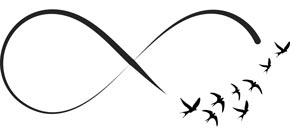
\includegraphics[width=0.44\textwidth]{./infinity.jpg}
  
  \vspace*{2\baselineskip}
  \textit{``fides in stellis, virtus in numeris"}
  
  \pagebreak
  
  \endgroup
}

\begin{document}

\title{\rmfamily\normalfont{Nexus: Een Peer-to-Peer Netwerk}}

\date{4 juli 2017}
    
\maketitle

\begin{abstract}

\noindent{\textit{``Je verandert nooit dingen door de bestaande realiteit te bestrijden. Om iets te veranderen bouw je een nieuw model dat het bestaande model overbodig maakt"}}

\begin{center}
R. Buckminster Fuller
\end{center}
\bigskip

\noindent{Door de geschiedenis heen zijn we getuige geweest van veel veranderingen in onze cultuur, technologie en bestuur.}
Deze veranderingen worden gevoed door de noodzaak voor de verdere evolutie van de mensheid. Nu benadert de mensheid een nieuw cruciaal punt waarin we de manier van werken volledig moeten veranderen; daarom hebben we Nexus gebouwd. Peer-to-Peer-technologie is de ruggengraat van een wereldwijde op blockchain gebaseerde cryptocurrency vertegenwoordigd door de ticker: \textit{NXS} die wereldwijd wordt verhandeld als alternatieve valuta met het vermogen om te concurreren met wereldeconomie\"en. Het Nexus framework maakt gebruik van een nieuw gedistribueerd database ontwerp, wiskundige algoritmes,
gemeenschapsbestuur, op de grond gebaseerde mesh-netwerken en een \textit{Low Earth Orbit} satelliet netwerk. 
Wij zijn Nexus, een connectie van mensen,
idee\"en en computers met als doel meer vrijheid te bieden. 
Welkom in de toekomst.

   
\end{abstract}

\newpage

\tableofcontents
\newpage
\maketitlepage
  {kSmith, pSmith, jSmith}


\paragraph{\textbf{\textit{Genesis} White Paper} - \textit{1.0.4} - Laatste Revisie 28 november 2017  }

\paragraph{}



\begin{wrapfigure}[4]{l}{0.40\textwidth}
    \centering
    \vspace{-25pt}
    \hspace{-15pt}
    
\includegraphics[width=0.30\textwidth]{./images/IMG_1228.JPG}
\end{wrapfigure}

\epigraph{nexus: een verbinding of reeks van verbindingen die twee of meer dingen met elkaar verbinden.}{\textit{\footnotesize{Oxford Engels woordenboek}}}

\section{Inleiding}

Peer-to-peer netwerken vormen de basis van digitale industrie\"en in de wereld. Dit ecosysteem blijft evolueren door innovators in de sector van open-source protocollen, zoals \textit{Bitcoin, BitTorrent, TOR, and IPFS}.
Het nut van deze netwerken heeft een steeds groter effect op mensen over de gehele wereld. Voor de eerste keer in de geschiedenis kan de overdracht van waarde plaats vinden zonder de noodzaak van tussenpersonen.
Nu, bijna tien jaar na de release van Satoshi Nakamoto's \textit{Bitcoin: een peer-to-peer elektronische valuta systeem} \cite{bitcoin} dat debuteerde op een Cypher Punk e-maillijst in een tijd van economische crisis, er veel voordelen zijn gerealiseerd, waaronder maar niet beperkt tot: \textbf{\textit{viz.}} verbeterde financi\"ele zekerheid, emancipatie van gecentraliseerde banksystemen, en de mogelijkheden voor nieuwe toepassingen op blockchains. Er zijn echter vele uitdagingen ge\"identificeerd zoals schaalbaarheid, consensus updates en overwegingen voor het post-quantum tijdperk dat zeer dichtbij is. Door oplossingen te bieden aan een ​​aantal van deze ge\"identificeerde problemen heeft Nexus het blockchain protocol verbeterd, waardoor een solide basis wordt gelegd voor de digitale economie van de toekomst. 
\bigskip

\subsection{Wat is Nexus?}
Nexus is een verbinding, of reeks van verbindingen van computers, bedrijven en mensen die de focus leggen op het opzetten van nieuwe financi\"ele toepassingen, technologie\"en, dienstverlening en soevereiniteit.  

\subsection{Wat is een blockchain?}

Een blockchain is een gedecentraliseerde en onveranderlijke openbare database van transacties. De database is georganiseerd door een reeks van blokken met elkaar te verbinden. Elk blok bevat een aantal transacties.
De blokken worden gerangschikt op tijd en aan elkaar gekoppeld met behulp van cryptografische hashes.\footnote{"Een cryptografische hash-functie is een functie die een invoer (of 'bericht') neemt en een alfanumerieke tekenreeks van vast formaat oplevert. De string wordt de 'hash-waarde' genoemd"\cite{wikihash}}\footnote{Het concept van een cryptografische reeks blokken stamt uit de Ehrsam, Meyer, Smith en Tuchman's uitvinding van Cipher Block Chaining (CBC) in 1976 \cite{cbc}. NB: dit is verschillend van \textit{blockchain} die hier op verschillende manieren wordt besproken, vooral omdat het geen proof-of-work bevat.}
Het berekenen van deze hashes vergt enorme computerkracht.\footnote{Dit wordt in het algemeen Proof-of-Work genoemd, maar omvat ook de innovatie van Sunny King: Proof-of-Stake \cite{peercoin}.} Elke blok bevat de hash van het vorige blok: \textit{op deze manier worden de blokken met elkaar gelinkt}.

\begin{center}
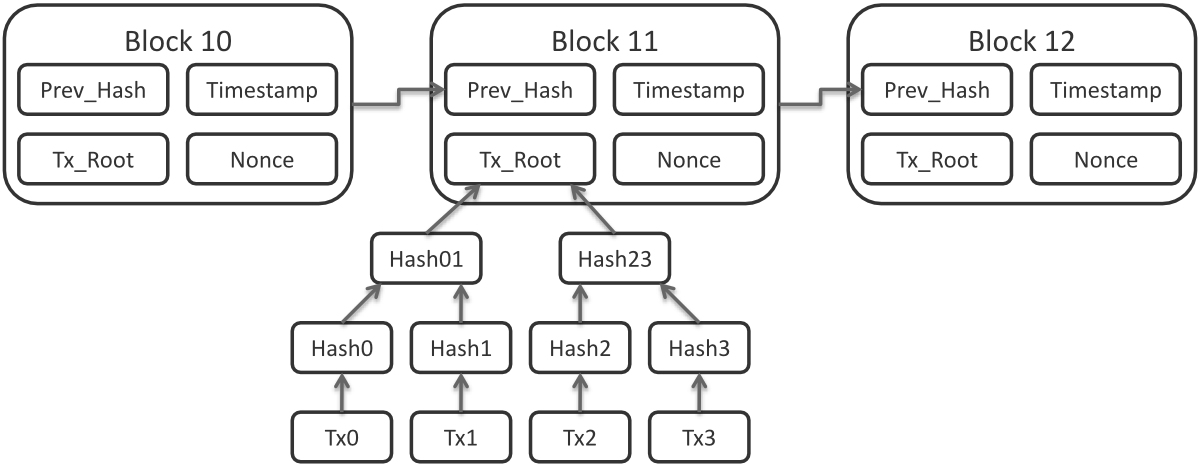
\includegraphics[width=0.80\textwidth]{./blockchain.png}
\end{center}
De blokken worden in intervallen geproduceerd en vormen een ketting van verifieerbare blokken die de transactiegeschiedenis bevatten. Deze gegevens kunnen niet gewijzigd worden zonder het werk van de \textit{voorgaande blokken} en \textit{bevestigingen} opnieuw uit te voeren.
Het eindresultaat is \'e\'en enkele, onveranderlijke ketting van transacties gegroepeerd door middel van in tijd geordende blokken die zijn gedistribueerd en geverifieerd door alle nodes in het netwerk.

\subsection{Hoe worden blokken gemaakt?}

Blokken worden gemaakt in een gedistribueerd netwerk van mijnwerkers \textit{(mensen die hun computers of speciale hardware in zetten om hashes te berekenen)} in een proces dat minen of in het nederlands mijnen wordt genoemd.
Om het in mensentaal te zeggen, stel je voor dat veel mensen in een kamer zitten en gemotiveerd zijn om een ​​prijs te winnen als ze de eerst zijn om de Rubik's puzzel op te lossen. De tegels van de Rubik's puzzel kunnen worden aanzien als transacties, waarbij een van de tegels de prijs \textit{(mint)} vertegenwoordigt die de winnaar mag claimen als hij de puzzel als eerst heeft opgelost. 
Ze mogen slechts \'e\'en willekeurige aanpassing doen per iteratie en worden beperkt door de snelheid van hun handen \textit{(sommige zijn sneller dan andere)}.
Uiteindelijk zal \'e\'en speler eindigen met een opgeloste puzzel. Wanneer men de oplossing vindt, wordt deze aan de andere spelers in de ruimte getoond. Als de andere spelers onafhankelijk verifi\"eren dat de puzzel correct is opgelost, wordt de winnaar beloond met de prijs en begint een nieuwe ronde.

\subsection{Zijn blockchains de oplossing?}

Blockchains zijn noodzakelijker nu we ons bewust worden van de uitdagingen waar we voor staan ​​in onze huidige samenleving. Door open te staan voor de uitdagingen worden we ons bewust van de beperkingen die legale monetaire systemen niet kunnen oplossen. We zien dat \textit{blockchains} veel monetaire uitdagingen oplossen, zoals ongecontroleerde inflatie, centrale banken en vele anderen. Toch zijn ze slechts een deel van de oplossing voor onze huidige economische omstandigheden.

\epigraph{Kwantitatieve versoepeling of vrijer vertaald kwantitatieve geldverruiming is een vorm van directe geldschepping door een centrale bank, waarbij deze effecten (zoals staatsobligaties) aankoopt met voor dat doel gecre\"eerd geld.}{\textit{Investopedia}}

\vspace{-138pt}
\hspace{-25pt}
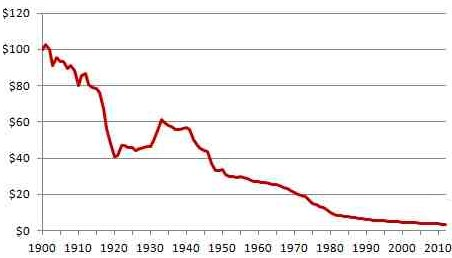
\includegraphics[width=0.60\textwidth]{./images/us-dollar.jpg}
\vspace{5pt}

\noindent
De term \textit{blockchain} moet niet verward worden met een versleutelde database (encryptie). De Dollar of Euro is in wezen een online virtuele valuta die gecodeerd is tussen banken die kan ingewisseld worden voor \textit{papieren geld}. Dit maakt de Dollar of Euro echter niet tot een blockchain. Wat een blockchain tot een echte blockchain maakt, is een gedecentraliseerd publiek beschikbaar dagboek (ledger)  zonder centrale autoriteit. 
Door een bepaald deel van een cryptocurrency te bezitten, bewijst u gedeeltelijk eigenaarschap in het financi\"ele systeem.


\subsection{De uitdagingen van geld}

De toepassing en implementatie van alle monetaire systemen in de wereld is een van de grootste uitdagingen waar we vandaag de dag voor staan. Dit is te wijten aan de vele wereldwijde beleidslijnen die ontworpen zijn om centrale banken in staat te stellen valuta's te cre\"eren als schulden met bijbehorende rente. Centrale banken hebben de mogelijkheid om de wereldeconomie\"en te be\"invloeden door de rentetarieven te veranderen, massa's geld te drukken \textit{(ook bekend als inflatie of hyperinflatie)}, kwantitatieve versoepeling of door verschillende andere vormen van kredietcreatie. Er zijn veel historische voorbeelden van centrale autoriteiten die deze enorme macht misbruikt hebben en dit allemaal ten koste van mensen die van deze instellingen afhankelijk waren. Voorbeelden hiervan zijn de hyperinflatie die opliep tot 30,000\% per maand in Duitsland na de eerste wereldoorlog, de Grote Recessie in Zimbabwe van het afgelopen decennium met bijna 79 miljard procent inflatie per maand en Hongarije na de tweede wereldoorlog, met inflatiecijfers van bijna \textit{13,000,000,000,000\%} per jaar.  \footnote{De geschatte 200\% per dag inflatie komt overeen met ongeveer dertien miljard percenten jaar \cite{hyperinflation}}


\section{Nexus}

Bij het bieden van de fundamentele basis voor verandering en vrijheid moeten meerdere componenten overwogen worden. 
Het volgende is een korte schets van de hoofdcomponenten die de basis vormen van Nexus.

\subsection{Hardware}

Nexus onderzoekt en ontwikkelt drie soorten netwerken die samenwerken om een ​​nieuw telecommunicatiesysteem te vormen. Deze worden beschreven in de onderstaande paragrafen.

\newpage

\subsubsection{Mesh Netwerken}

\begin{wrapfigure}[14]{l}{0.44\textwidth}
    \centering
    \vspace{-20pt}
    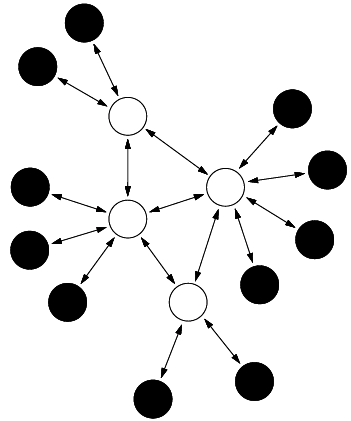
\includegraphics[width=0.44\textwidth]{mesh.png}
\end{wrapfigure}

Een mesh netwerk is een netwerktopologie waarbij elk knooppunt gegevens doorgeeft. Alle netwerk knooppunten werken samen bij de distributie van gegevens in het netwerk \cite{meshnetworks}.\\ 

\noindent 
Dit maakt de groei mogelijk voor netwerken op de aarde om gegevensuitwisseling in gelokaliseerde gebieden af ​​te handelen.\\

\noindent Deze mesh netwerken op de aarde zelf zullen veel telecommunicatie problemen oplossen. Gespecialiseerde antennes kunnen door mensen aangekocht en bedient worden, waardoor er netwerken worden gevormd die eigendom zijn van de personen die het gebouwd hebben.

\subsubsection{Cube Satellites}

Cube satellites of in het nederlands mini satellieten in de vorm van een kubus maken deel uit van het mesh netwerk dat naarmate de groei de problemen met 'line of sight' en transcontinentale communicatie moeten overwinnen. Dit probleem kan worden opgelost met een geheel van satellieten die ontworpen zijn om de caching \footnote{Een cache (spreek uit: kesj of kasj, van het Engelse woord 'cache', voorraad of opslagplaats) is een opslagplaats waarin gegevens tijdelijk worden opgeslagen om sneller toegang tot deze data mogelijk te maken.\cite{caching}} laag te voorzien in de ruimte voor het mesh netwerk dat op zijn beurt gegevens uitwisselt met het mesh netwerk dat zich op de aarde bevindt.

\subsubsection{Grondstations}

Grondstations zorgen voor de satelliet \textit{up en downlinks}. 
Deze zijn verantwoordelijk voor caching van gegevens op de aarde, het draaien van een nexus daemon en het defini\"eren van een route om gegevens door te sturen naar een geadresseerd eindpunt.

\subsection{Software}

Er zijn veel soorten softwaretoepassingen die een integraal onderdeel zijn van de functionaliteit en effici\"entie van Nexus. De softwaresystemen worden voortdurend ontwikkeld en verbeterd naarmate Nexus groeit.

\begin{itemize}
\item \textbf{Daemon (achtergrond proces)}

Nexus werkt op een low-level software applicatie die we de \textit{"Nexus Daemon"} noemen.
Verschillende instanties van deze softwaretoepassing communiceren met elkaar en vormen een peer-to-peer-netwerk. Ze wisselen gegevens uit in de vorm van transacties en beveiligen ze in een gedistribueerde database die een blockchain wordt genoemd.

\item \textbf{Wallet (portemonnee)}

Een command line en een grafische Qt versie van de Nexus wallet zijn momenteel beschikbaar \cite{githubnexusreleases} \cite{nexusearth}.
De nieuwe versie van de Nexus wallet zal een grafische toepassing van hoger niveau zijn die toegang biedt tot de functies van de \textit{``Nexus Daemon"} via een HTML / JS-interface. 
De interface fungeert ook als modulair framework waarin modules kunnen worden ontwikkeld voor een betere gebruikerservaring.\footnote{Dit is wordt actief ontwikkelt op het moment van dit schrijven.}

\item \textbf{Library (bibliotheek)}

De lower-level library bestaat uit drie delen, namelijk Crypto, Databank en Protocol. Ze vormen een basislaag van programmeer sjablonen die kunnen  gebruikt worden om er complexere klassenstructuren bovenop te maken. 

\end{itemize}

\section{Specificaties}

Dit gedeelte bevat details over de belangrijkste softwarecomponent van Nexus, de \textit{"Nexus Daemon"}.
Deze software component is de basis voor het Nexus netwerk en houdt rekening met juiste uitgaves, mining, trust en andere componenten van beveiliging en effici\"entie.
 

\subsection{Hashing}

Hashing is een cruciaal onderdeel van elke cryptocurrency. 
De recente SHA-1 botsing computatie die door Google werd ontdekt benadrukt de nood aan veiligere hashes \cite{googlesha1}. 
Een van de innovaties van Nexus is het gebruik van nieuwe hashing-functies met als doel een verbeterde beveiliging.

\subsubsection{SHA-2}

SHA-256 is lid van de SHA-2, een set van cryptografische hashfuncties.\footnote{SHA staat voor Secure Hashing Algorithm.}
Het is ontworpen door de National Security Agency (NSA) en in 2001 gepubliceerd \cite{wikisha2}.
SHA-256 wordt gebruikt in Bitcoin-mining en bij het maken van Bitcoin adressen \cite{bitwiki256}.

\subsubsection{SHA-3}

Nexus gebruikt een nieuwer, veiliger hashing algoritme dan dat van Bitcoin. 
De SHA-3 \cite{sha3} standaard was het resultaat van een wedstrijd \cite{nistcompetitionend} met als doel een alternatief voor SHA-2 op te leveren. Deze wedstrijd werd georganiseerd door het National Institute of Standards and Technology (NIST). 
De winnaar van deze wedstrijd werd in 2012 geselecteerd. 
Het nieuwe algoritme SHA-3 is een subset van de cryptografische familie Keccak \cite{nistgovk}.

\subsubsection{Skein}

Het Skein-algoritme was de nummer twee in de NIST hashfunctie competitie \cite{wikiskein}.
Deze wordt ook gebruikt in Nexus in combinatie met SHA-3. Het voordeel van deze aanpak is een grotere diversiteit in veilige hashing functies die in Nexus worden gebruikt.

\begin{wrapfigure}{r}{0.50\textwidth} %this figure will be at the right
    \caption{Vier van de 72 ronden van het Threefish-512 blokcijfer dat in Skein gebruikt word \cite{skeinpaper}.}
    \centering
    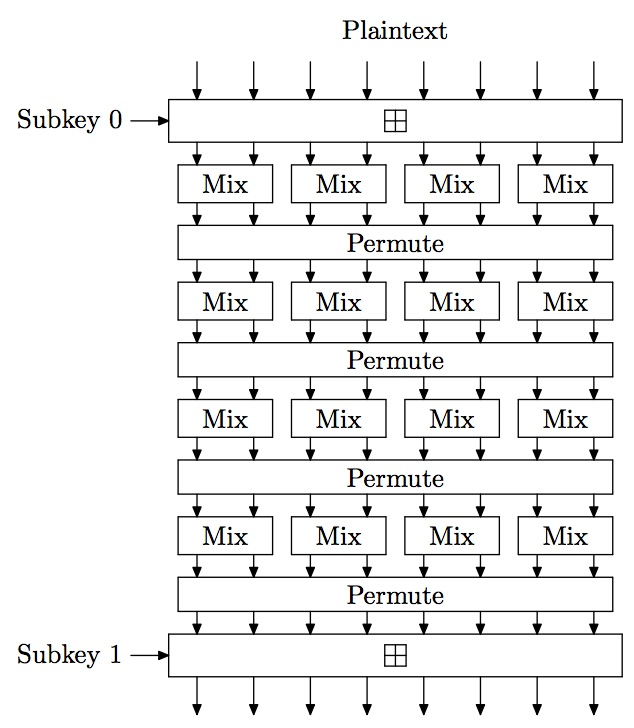
\includegraphics[width=0.50\textwidth]{skein-threefish-512-part.jpg}
\end{wrapfigure}

\pagebreak
\subsubsection{Skein-Keccak}

Nexus hashing is opgebouwd uit twee veilige hashing algoritmen: Skein en Keccak \cite{sha3announce}. 
Deze twee algoritmen worden gecombineerd om \'e\'en enkele SK-1024 (Skein-Keccak 1024 bit) hash te vormen. 
Er zijn drie soorten uitvoer lengtes in Nexus hashing: SK-256, SK-512 en SK-1024. Publieke sleutels zijn gehashed met SK-256 om ze te beschermen tot ze worden gebruikt. 
Transacties worden gehashed met SK-512 terwijl SK-1024 wordt gebruikt voor de proof-of-work hash.

\subsubsection{Vergelijking van 256 bit en 1024 bit}

Het volgende voorbeeld illustreert het verschil in grootte tussen een Nexus blok hash en een Bitcoin blok hash:

\begin{itemize}
\item Bitcoin Hash (256 bit)
\begin{lstlisting}
00000000000000000478710bb73175549d34893a375
454df1af122c26a453d9b
\end{lstlisting}

\item Nexus Hash (1024 bit)

\begin{lstlisting}
0000000001370e3764cffad92091c99b5beaf85f6fc
edae66e77be9de6f0ce6e3d8b1da4b6581d35f3ff6c
f359b10ab85c3b226f41cf864c979e8492f854c56d3
0e329ffc012c338caa7f3c6197137afb1637adc0b2f
22270990d0034c0ea0eae306ec28b7a565a1459896d
69a1c20f9f63af6c5fd672d76c6c8934e8363a21
\end{lstlisting}
\end{itemize}


\pagebreak
\subsection{Uitgave}

Emission of in het nederlands 'uitgifte'. In Bitcoin is een vaste hoeveelheid BTC beschikbaar als beloning voor mijnwerkers (miners) in elk blok. Dit bedrag halveert om de vier jaar, waardoor de inflatie van Bitcoin afneemt. Deze plotselinge verandering in de beloning per blok is echter een schok voor de markt. Mijnwerkers (miners) spenderen grote sommen geld aan apparatuur en personeel. Als de beloning per blok halveert, wordt hun winst gehalveerd.
\footnote{Deze winstdaling kan in theorie voorzien worden zodat mijnwerkers (miners) zich kunnen voorbereiden. Het is realistisch gezien moeilijk voor mijnwerkers (miners) om dit te verantwoorden in een snel veranderend systeem.}
Een dergelijke onzekerheid kan mogelijk een negatief effect hebben op de netwerkbeveiliging \cite{cdhalving}.
\noindent Nexus verbetert dit model door de beloning bij elk blok aan te passen. Gebruikmakend van de vergelijkingen voor exponentieel verval \textit{(met een zorgvuldig gekozen constante $k$)}, ($e^{-kt}$), 
wordt elke minuut een aanbetaling in reserves gedaan. Het reserve bepaalt de beschikbare beloning voor mijnwerkers (miners).\\ 

\noindent De beschikbare hoeveelheid is op tijd vergrendeld en niet op de productie van blokken. Inconsistente blocks hebben geen effect op de beschikbare hoeveelheid. Dit maakt het mogelijk de beschikbare hoeveelheid nauwkeurig te berekenen op elk moment na een netwerk tijdslot.

\subsubsection{Reserves}

Een traditioneel waterreservoir bevat water dat door een stad kan worden gebruikt. De totale hoeveelheid water die de stad kan gebruiken, is beperkt op basis van de hoeveelheid water in het reservoir. Op vergelijkbare wijze bepaalt het reservesysteem van Nexus hoeveel NXS beschikbaar is voor mijnwerkers (miners) op een bepaald moment.\\ 

\noindent Er zijn drie reserves. De hoeveelheid NXS die in elke reserve wordt gestort, wordt wiskundig bepaald door \textit{vervalvergelijkingen}.

\begin{equation}\label{eq:reserves}
\resizebox{.75\hsize}{!}{$
\begin{array}{ll}
      V_{d} = \;\;1 \cdot e^{-0.00000059 \cdot T_{m}} & + 0.032 \\
      V_{a} = 10 \cdot e^{-0.00000055 \cdot T_{m}} & + 1 \\
      V_{m} = 50 \cdot e^{-0.0000011 \cdot T_{m}} & + 1 \\
\end{array} $}
\end{equation}

\noindent Waar $T_m$ de tijd is in minuten en $V_{d}$, $V_{a}$, $V_{m}$ zijn de reserve stortingen voor mijnwerkers (miners), ambassadeurs en ontwikkelaars.

\pagebreak
\subsubsection{Beloningen}

De beloningen worden berekend op basis van de reservewaarde. 
Dit voorkomt uitgave voorbij het streefniveau.
\noindent Deze drie vergelijkingen beschrijven de intervallen waarin de blokbeloning $V_{b}$ verandert op basis van reservewaarden $V_{m}$ bij $T_{m}$ door de $T_{m}$ waarde uit vergelijkingen te comprimeren \ref{eq:reserves}.

\begin{equation}
\resizebox{.60\hsize}{!}{$
    V_b= 
\begin{cases}
    \frac{T_{a}}{60} \cdot V_{r}, & T_{m} \leq 2.5\\
    2.5 \cdot V_{r}, & 2.5 < T_{m} < 20\\
    3.0 \cdot V_{r}, & T_{m} \geq 20
\end{cases}
$}
\end{equation}

\begin{center}
Waar $T_a$ de werkelijke tijd is, $T_o$ de offset tijd is en $T_t$ de doeltijd is.\\
\end{center}


\subsubsection{Intrest of ook Rente (Minting)}

\begin{wrapfigure}{r}{0.50\textwidth}\label{fig:interestrate} %this figure will be at the right
    \centering
    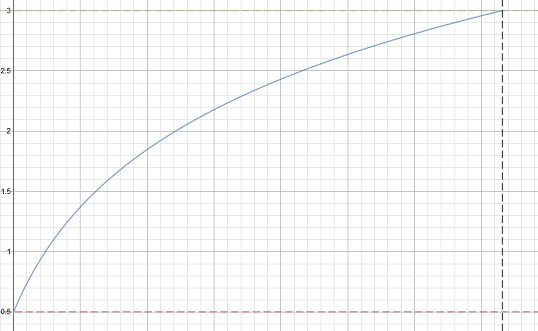
\includegraphics[width=0.50\textwidth]{interest.png}
    \caption{Rentevoet Grafiek.}
\end{wrapfigure}

Peer-to-peer-netwerken, zoals Bitcoin en Nexus, vereisen de ondersteuning van vele knooppunten over de hele wereld. Als er niet genoeg knooppunten zijn, lijden netwerk stabiliteit, decentralisatie, snelheid en beveiliging. Bitcoin zit met het probleem\footnote{Dit is een economisch probleem waarbij elk individu het meeste profijt probeert te trekken uit een bepaald middel\cite{tragedycommons}.}
\noindent waarbij iedereen wil dat meer mensen een peer-to-peer-wallet draaien, maar er is weinig stimulans om het effectief te doen. Nexus lost dit probleem op door mensen te belonen met nieuwe munten om hun portemonnee 24/7 beschikbaar te houden en als knooppunt in het netwerk te fungeren. Om het simpel te zeggen: als iemand de Nexus portemonnee op zijn computer installeert en er voldoende NXS insteekt, dan zullen ze af en toe een blok vinden en extra NXS verdienen.\footnote{ Dit is een manier om het netwerk te ondersteunen en Nexus te verdienen zonder kostbare en moeilijk te bedienen hardware en software voor het genereren van munten (minen).}\\

\noindent Dit systeem beloont deelnemers naarmate hun bijdrage aan het netwerk. Als iemand blokken produceert door deze methode te gebruiken, groeit zijn of haar vertrouwens score. Bij een hogere vertrouwens score komt een hogere intrest (minting rate). De intrest (minting rate) $R_m$ varieert van 0.5 \% tot 3 \%.

\paragraph{}
\begin{equation}
\resizebox{.65\hsize}{!}{$R_m = \frac{0.025 \cdot ln(\frac{9 \cdot a_{t}}{31449600} + 1)}{ln(10)} + 0.005$}
\end{equation}

\noindent Waar $a_t$ de leeftijd is van uw vertrouwens score (het aantal seconden sinds de Genesis transactie waarbij de Trustkey werd genereerd).

\subsection{Blok validatie}

Er zijn drie manieren om een ​​geldig Nexus blok te maken en nieuwe NXS te genereren. Er zijn twee proof-of-work kanalen en een kanaal met proof-of-holdings (bewijs van bewaring). De proof-of-work kanalen zijn het “Prime Channel” (Priemgetallen) en het “Hashing Channel”. In het “Prime Channel” zoeken mijnwerkers (miners) naar priemgetallen van ~308 cijfers groot.
In het hash channel, wordt de standaard Hashcash \cite{hashcash} werkwijze gebruikt door middel van het SK-1024 hashing algoritme. 
De twee proof-of-work-kanalen voorkomen dat er te veel blokken achter elkaar worden geproduceerd, waardoor een 51\% aanvaller over beide kanalen wordt gedwongen.\footnote{Reserves tussen Prime en Hash worden gelijk verdeeld, elk 50 \%}

\subsubsection{Priemfactoren}

Het doel van het werk in het Prime Channel is een zoektocht naar priemfactoren \cite{wikiprimecluster}.\footnote{De cijfers die in deze zoekopdrachten worden gevonden, zijn eigenlijk waarschijnlijke priemgetallen \cite{wikiprobable}. Ze doorlopen de Fermat Prime test \cite{wikifermat} op basis 2, 3 en 5.}
Het vinden van deze priemfactoren is een proces van vallen en opstaan. Mijnwerkers (miners) moeten vele getallen proberen om er een te vinden die het begin is van een priemfactor \cite{wolframprimecluster,primesolominer}.\\ 

\noindent Het aantal priemgetallen in een priemfactor wordt de kettinglengte genoemd.
\footnote{De ``ketting" hier moet niet worden verward met de ketting in de blockchain.}
Een priemfactor met een langere ketting is moeilijker te vinden dan een met een kortere ketting. Het eerste priemgetal in de keten moet hoger zijn dan de block hash en kleiner dan de block hash plus $2^{64}$.\footnote{De block hash kan niet a priori worden bepaald voor toekomstige blokken omdat deze gebaseerd is op eerdere blok informatie. Daarom moet een mijnwerker (miner) het zoeken naar hun priemfactor opnieuw starten nadat elk nieuw blok is gevonden}
Als de eerste priemgetallen in het cluster aan deze criteria voldoen, wordt dit als een geldige oplossing beschouwd.\\

\noindent Een voordeel van het zoeken naar priemfactoren is dat er wordt aangenomen dat het resistent is tegen GPU-, FPGA- en ASIC-mining in tegenstelling tot hashing. Een andere voordeel is dat de door de mijnwerker (miners) geproduceerde gegevens nuttig zijn voor wiskundig onderzoek naar priemgetallen \cite{findingprimeclusterspaper} \cite{nxsprimecom}.
De toepassingen van priemgetallen onderzoek kunnen verder reiken dan de wiskunde en de kwantumfysica \cite{physicsmathprime}.
Dit is een van de manieren waarop Nexus waarde toevoegt aan de wetenschap en de wereld.

\subsubsection{Hashing}

Het hashing channel maakt gebruik van \textit{Hashcash} \cite{hashcash} proof-of-work.
Mijnwerkers (miners) voeren code uit \cite{skminer,wolfniro} op GPU's in een poging een hash te vinden die aan een bepaalde moeilijkheidsgraad voldoet. Als ze geluk hebben, vinden ze een hash met minstens een bepaald aantal 0 bits in het begin. Dit betekent dat de hash wordt voorafgegaan door een aantal 0'en en een kleiner geheel getal is. Dit wordt een "gedeeltelijke botsing" genoemd. Dit is vergelijkbaar met de proof-of-work die Bitcoin gebruikt. Bitcoin gebruikt SHA-256 terwijl Nexus de nieuwere SHA-3 gebruikt in combinatie met Skein.


\subsubsection{Stockeren}

Proof-of-Holdings \textit{(POH)} biedt een derde beveiligings kanaal. Een aanvaller zou 51 procent van de NXS voorziening nodig hebben om dit kanaal aan te vallen in combinatie met de hash- en prime-kanalen. Door deel te nemen aan dit systeem wordt je beloond voor het actief ``bijhouden" van je munten, de beloning is uiteraard nieuwe munten. Dit betekent dat het netwerk gebruikers stimuleert om bij te dragen aan de beveiliging van het systeem. Dit zorgt voor een natuurlijke groei van het aanbod van munten in de loop van de tijd, wat zeer bevorderlijk zal zijn voor het netwerk, de economie en gebruikers.\\ 

\noindent In tegenstelling tot de huidige modellen van de Centrale Bank, gaat dit nieuwe aanbod munten rechtstreeks in handen van de gebruikers in plaats van te worden gefilterd door een fractioneel reserve systeem. Bovendien hebben deze nieuw geslagen munten geen schuld in verband met hun uitgifte en hoeven ze daarom nooit terug te worden betaald aan het systeem met bijbehorende rente, zoals het geval is met veel huidige valuta's. De wisselkoers is vastgesteld als een variabele rente tussen 0.5\% en 3\% om een ​​kleine natuurlijke groei aan de munt voorraad toe te staan met als doel de economische mogelijkheden te vergroten.

\subsection{Moeilijkheidsgraad (Difficulty)}

De moeilijkheid om een ​​blok te vinden, wordt bij elk nieuw blok aangepast. Het moeilijkheids algoritme dat Nexus gebruikt combineert gewogen gemiddelden voor de laatste $n$ blokken.
Een gewogen gemiddelde tijd, $T_a$ wordt als volgt berekend:\\ 

\begin{equation}
\resizebox{.75\hsize}{!}{$T_{a} = \frac{\sum_{i=1}^{n} w \cdot i [ T_b(H - n + i) - T_b(H-n+i-1) }{n}$}
\end{equation}\\ 

\noindent Waar $H$ huidige blok moeilijkheid is, $T_b$ is de blok tijdsindicatie op een gegeven moeilijkheid, $n$ is de blockchain diepte en $w$ is een gewichts constante (momenteel ingesteld op 3).\\  

\noindent $Mod_d$ is de factor die wordt gebruikt om de moeilijkheidsgraad te wijzigen\\ 

\begin{equation}
\resizebox{.70\hsize}{!}{$
    Mod_d= 
\begin{cases}
    [1 - (Min_{d} \cdot T_{o})] \cdot T_{t}, & \text{if } T_{a} \geq T_{t}\\
    [1 + (Max_{d} \cdot T_{o})] \cdot T_{t}, & \text{otherwise}
\end{cases}
$}
\end{equation}

\noindent Waar $T_t$ de streeftijd, $T_o$ is de offset tijd, $Min_d$ is de minimale moeilijkheidsgraad vermindering en $Max_d$ is de maximale moeilijkheidsgraad verhoging.

\epigraph{Het is een ondeugd om iedereen te vertrouwen, evenveel als een ondeugd om niemand te vertrouwen.
}{\textit{\footnotesize{Seneca}}}

\pagebreak
\subsection{Vertrouwen (Trust)}\label{subsection:Trust}

Vertrouwen of Trust is een kern component van Nexus. Knooppunten (of zoals hierboven aangehaald deelnemers) die een gevestigd belang hebben in en ten goede komen aan het gehele netwerk door consistent deel te nemen, worden als betrouwbaarder beschouwd. Op dit moment wordt vertrouwen verdiend door Nexus in een portefeuille te houden en regelmatig geldige blokken te genereren. Dit verdiend vertrouwen wordt vastgelegd in de Nexus blockchain en is gekoppeld aan een vertrouwens code.\\ 

\noindent Toekomstig onderzoek en de ontwikkeling van Nexus zal zich concentreren op het op vele manieren gebruiken van het concept van vertrouwen. Met behulp van vertrouwen kan een nieuw beveiligingsmodel ontwikkeld worden. De kracht van de Nexus economie en de betrouwbaarheid ervan zal versterkt worden door de het vertrouwen tussen de vrijwillige interacties met individuen en groepen van individuen.

\subsubsection{Gewicht (Weight)}

Gewicht bepaalt de snelheid waarmee kan worden gezocht naar nieuwe vertrouwens blokken. Het komt in de vorm van twee verschillende gewichts variabelen: Blok gewicht ($W_b$) en Vertrouwen gewicht ($W_t$).

\begin{equation}
W_{t} = Min(17.5, \frac{16.5 \cdot ln(\frac{2 \cdot a_t}{2419200}) + 1}{ln(3)} + 1.0)
\end{equation}

\begin{equation}
W_{b} = Min(20.0,\frac{19.0 \cdot ln(\frac{2 \cdot a_b}{86400}) + 1}{ln(3)} + 0.05)
\end{equation}

\noindent Waar $a_t$ de vertrouwens leeftijd is en $a_b$ de leeftijd van de block.

\subsubsection{Drempel (Threshold)}

Er is een systeem ontwikkeld om een op tijd gebaseerd ​​energie effici\"ent vertrouwen systeem mogelijk te maken. Dit wordt geregeld door de Energie Effici\"ente Drempel (Energy Efficiency Threshold) $E_t$.

\begin{equation}
\resizebox{.22\hsize}{!}{$E_{t} = \frac{100 \cdot T_{a}}{N_{once}}$}
\end{equation}

\pagebreak
De vereiste drempelwaarde $R_t$ is

\begin{equation}
\resizebox{.5\hsize}{!}{$R_{t} = \frac{(50 - W_{t} - W_{b}) \cdot 1000}{C}$}
\end{equation}

Waarbij C de totale NXS is in een vertrouwens transactie.

\subsubsection{Vertrouwenssleutel (Genesis)}

De genesis transactie is de eerste transactie van een vertrouwens sleutel. Deze bepaald de beginleeftijd van de vertrouwens sleutel en dient vervolgens om een ​​referentie te krijgen over zijn huidige gewicht en de bijbehorende intrest. De hash van deze genesis transactie kan daarom worden gebruikt als invoer in toekomstige transacties om te verifi\"eren dat een vertrouwens blok gekoppeld is aan een bijbehorende genesis transactie.

\noindent De volgende vergelijking beschrijft het genesis gewicht dat vereist is om een ​​drempelwaarde te bereiken die hoog genoeg is voor een genesis transactie te cre\"eren met bijbehorend blok.\footnote{Genesis transactie gewicht omvat niet het blok gewicht.}

\begin{equation}
\resizebox{.70\hsize}{!}{$
W_{g} = Min(17.5, \frac{16.5 \cdot ln(\frac{2 \cdot a_{c}}{7257600}) + 1}{ln(3)} + 1.0)
$}
\end{equation}

\noindent Waarbij $a_c$ de munt leeftijd is van de gebruikte munten.

\subsubsection{Interval (Intervals)}
 
Vertrouwens blokken kunnen niet met dezelfde vertrouwens sleutel worden gemaakt, tenzij het interval of het aantal blokken tussen hun laatste vertrouwens blok groter is dan $I_{t} \geq 6$.

\subsection{Tijdsverschil (Clock Drift)}

Clock drift verwijst naar verschillende gerelateerde verschijnselen waarbij een klok niet exact hetzelfde loopt als een referentie klok \cite{wikiclockdrift}.
Dit wordt meestal opgelost door verbinding te maken met een centrale server en / of een atoomklok. Nexus lost dit op met een peer-to-peer tijdregistratiesysteem dat alle klokken op het netwerk gesynchroniseerd houdt met een universeel tijd protocol.


\subsection{Beveiliging (Security)}

Bitcoin en andere cryptocurrencies staan tot maximaal 2 uur klok afwijking in de toekomst toe, wat betekent dat blokken tot 2 uur voorbij de huidige netwerk tijd (in het Engels \textit{timestamp}) kunnen gemaakt worden, waardoor potenti\"ele aanvalsvectoren ontstaan. 
Nexus bestrijdt deze synchronisatie problemen niet met de mediaan doorheen de tijd, zoals Bitcoin dat doet, maar eerder met een Unified Time systeem dat op protocol niveau werkt, zodat alle Nexus klokken tot op de seconde gesynchroniseerd zijn.

\subsection{Tijdslot (Time-Locks)}

Omdat de klokken in het Nexus netwerk worden gesynchroniseerd kunnen nieuwe regels in het protocol worden geactiveerd op basis van tijd stempels (in het Engels \textit{timestamp}) in plaats van bloknummers. Dit stelt netwerkdeelnemers in staat om consensus updates nauwkeuriger te activeren.


\subsection{Controlepunten (Checkpoints)}

Geautomatiseerde en gedecentraliseerde controlepunten worden elk uur gemaakt. Een controlepunt verhindert dat een blok die niet ontstaan is uit het laatste controlepunt ongeldig is. Dit voorkomt dat een aanvaller een alternatieve blockchain produceert die het vorige controlepunt vooraf gaat.

\bigskip
\epigraph{Ik denk dat ik gerust kan zeggen dat niemand quantummechanica	begrijpt.
}{\textit{\footnotesize{Professor Richard Feynman, 1965 Natuurkunde Nobelprijswinnaar \cite{nobelfeynman}}}}

\pagebreak
\section{Post-quantum-overwegingen}

\begin{wrapfigure}{r}{0.60\textwidth} %this figure will be at the right
	\vspace{-15pt}
    \centering
    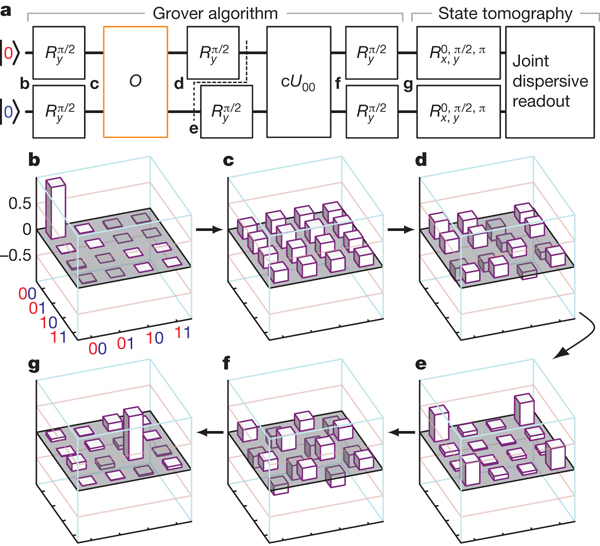
\includegraphics[width=0.50\textwidth]{grovers.jpg}
    \caption{Het algoritme van Grover over twee Qubits}
\end{wrapfigure}

\subsection{Algoritme van Grover}

Het algoritme van Grover is een quantum algoritme dat werd bedacht door Lov Grover in Bell Labo. De samenvatting in Grover's theorie uit 1996 biedt een nuttige beschrijving: "Stel je een telefoongids voor met N namen gerangschikt in willekeurige volgorde. Om iemands telefoonnummer te vinden met een waarschijnlijkheid van de helft, zal elk klassiek algoritme ... een minimum van $N/2$ namen moeten bekijken. Qubits kunnen in een superpositie van toestanden zijn, wat betekent dat een qubit een 0 of een 1 kan zijn. Als gevolg hiervan kan het gewenste telefoonnummer alleen worden verkregen in $O(\sqrt{N})$ stappen \cite{lovgrover}."\\ 

\noindent Het resultaat van een black box-functie kan worden gebruikt om\footnote{Op een probabilistische manier.} de invoer te bepalen.
Dit betekent dat de meeste eenrichtings cryptografische hashfuncties gevoelig zijn voor dit algoritme. 
En inderdaad, het algoritme van Grover kan een 256-bits sleutel door middel van brute force via $2^{128}$ iteraties de input berekenen.\\ 

\noindent Het algoritme gaat door met het oproepen van $G$ $[\frac{\pi}{4} \cdot 2^{\frac{k}{2}}]$ voor de verificatie van de subroutines. De grootste overhead in het algoritme van Grover is echter de kost van foutdetectie die klassiek moet worden uitgevoerd om de nauwkeurigheid van de qubits te garanderen (het overwinnen van kwantum ruis) en de twee subroutines van Grover iteratie te waarborgen.\\


\begin{table}[ht]
\caption{Vergelijking voor Grover zoekopdracht van SHA-256 en SHA3-256 \cite[p.~18]{groversalgorithm}}
\begin{center}
\begin{tabular}{c|ccc|}
    \hline
    \hline
    & & \textbf{SHA-256} & \textbf{SHA3-256} \\
    \hline
    \multirow{4}{*}{\rotatebox[origin=c]{90}{Grover}}
    &T-count & $1.27 \cdot 10^{44}$ & $2.71 \cdot 10^{44}$ \\
    &T-depth & $3.76 \cdot 10^{43}$ & $2.31 \cdot 10^{41}$ \\
    &Logical qubits & $2402$ & $3200$ \\ 
    &Physical qubits & $1.39 \cdot 10^{7}$ & $1.94 \cdot
    10^{7}$ \\
    \hline
    
    \multirow{4}{*}{\rotatebox[origin=c]{90}{Distilleries}}
    &Qubits per Distillery & $3600$ & $3600$ \\
    &Total Distilleries & $1$ & $294$ \\
    &Code Distilleries & $\{33, 13, 7\}$ & $\{33, 13, 7\}$ \\ 
    &Physical qubits & $5.54 \cdot 10^{5}$ & $1.63 \cdot
    10^{8}$ \\    
    \hline
    
    \multirow{4}{*}{\rotatebox[origin=c]{90}{Total}}
    &Logical qubits & $2^{12.6}$ & $2^{20}$ \\ 
    &Code Cycles & $2^{153.8}$ & $2^{146.5}$ \\
    &Total Cost  & $2^{166.4}$ & $2^{166.5}$ \\
    
    \hline
    \hline
\end{tabular}
\end{center}
\end{table}
%bdg% Table reviewed, matches info from referenced paper, page 18.

\noindent De eerste subroutine van $G$ probeert te beweren dat g : $\{0, 1\}^k \rightarrow \{1, 0\}$ alleen $X$ op $1$ toewijst als $f(x) = y$. 
De volgende subroutine wordt de \textit{``Diffusion Operator"} genoemd en implementeert de transformatie van g om de kans te vergroten dat $f(x) = y$.\\ 

\noindent Zoals ge\"illustreerd in Tabel 1 resulteert het algoritme van Grover in een reductie van bijna 50\% op de beveiliging geboden door one-way hashing functies tegen brute force aanvallen. Dit houdt in dat een hash, die twee keer zoveel bits heeft, gebruikt moet worden om hetzelfde niveau van beveiliging tegen brute force aanvallen te bereiken.


\subsection{Elliptische Curve cryptografie}

Elliptische curve cryptografie, in termen van klassiek computergebruik, behoudt hoge veiligheidsstandaarden met kleinere sleutelgrootten in vergelijking met RSA \cite{wikikeysize}.
De volgende vergelijking kan worden gebruikt om een ​​elliptische curve weer te geven:

\begin{equation}
\resizebox{.33\hsize}{!}{$y^2 = x^3 + ax + b$}
\end{equation}

%%Preston -Colin figure wrapping needs adjusted
\pagebreak
\subsection{Curve groepen en velden}


\begin{wrapfigure}[8]{r}{0.40\textwidth} %this figure will be at the right
\vspace{-40pt}
\caption{Illustratie van een elliptische curve}
    \centering
    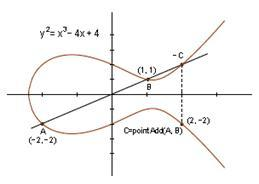
\includegraphics[width=0.40\textwidth]{ecc.JPG}
\end{wrapfigure}

In Nexus zijn de elliptische curve domein parameters gebaseerd op \textit{sect571r1} \cite{sect571r1}zoals gedefinieerd in de 'Standards for Efficient Cryptography 2: Recommended Elliptic Curve Domain Parameters' en deze worden gedefinieerd over een binair veld $\mathbb{F}_{2^m}$.
De domein parameters die in de meeste andere digitale valuta's worden gebruikt, zijn gebaseerd op \textit{secp256k1} \cite{secp256k1}. Deze parameters zijn geassocieerd met een Kolbitz curve en worden gedefinieerd over een priem veld  $\mathbb{F}_p$.

\subsection{Private sleutels (Private Keys)}

Een private key is een sleutel dat alleen aan de eigenaar van munten op een bepaald adres moet kennen. 
Als u een beveiligde private key wilt maken, moet u beginnen met een getal dat zo dicht mogelijk bij het echt willekeurige ligt.\footnote{Dit wordt afgehandeld door de Nexus portefeuille software - deze genereert private keys en bewaart ze.}
Als iemand kan achterhalen wat de priv\'esleutel is, kan hij of zij de munten verplaatsen naar een ander adres. Daarom is beveiliging van de private key zo belangrijk. U wilt niet dat iemand anders ontdekt wat uw 'geheime sleutel' is en u wilt niet dat zij het kunnen raden of bepalen met een complex algoritme op basis van openbare gegevens. Zowel Bitcoin als Nexus gebruiken grote getallen, zodat er bijna geen kans is dat iemand anders hetzelfde willekeurige nummer genereert en het onmogelijk is voor iedereen om alle nummers te proberen.\footnote{"Hoeveel nummers? Maak voor elke korrel zand op aarde een nieuwe aarde. Er zijn 26 miljard unieke Bitcoin adressen voor elke korrel zand op elk van die aardes. "\cite{weusesand} Omdat de sleutels in Nexus langer zijn, zijn er astronomisch meer mogelijke Nexus adressen.}
Bitcoin sleutels zijn 256 bits lang, terwijl de Nexus sleutels meer dan twee keer zo lang zijn namelijk 571 bits.

\bigskip
\textbf{Bitcoin Private Key (256 bit)}
\begin{lstlisting}
5Kb8kLf9zgWQnogidDA76MzPL6TsZZY36hWXMssSzNydYXYB9KF
\end{lstlisting}

\bigskip
\textbf{Nexus Private Key (571 bit)}
\begin{lstlisting}
6Wuiv513R18o5cRpwNSCfT7xs9tniHHN5Lb3AMs58vkVxsQdL4atHTF
Vt5TNT9himnCMmnbjbCPxgxhSTDE5iAzCZ3LhJFm7L9rCFroYoqz
\end{lstlisting}

\subsection{Publieke sleutels (Public Keys)}

Het is eenvoudig om een public key te bepalen van een private key, maar niet omgekeerd. Wanneer u een betaling van iemand vraagt, ontvangt u eerst een \textit{Nexus address} van uw portemonnee.
 Dit adres is niet uw public key, dit wordt een publieke sleutel hash of \textit{PKH} genoemd.
Zoals de naam al aangeeft, is deze gemaakt door uw public key te hashen en deze te converteren naar Base58 codering. Dit betekent dat een aanvaller die eerst uw private key wil achterhalen uw public key moet bepalen via de \textit{PKH}.
Gelukkig is dit een onoverkomelijk probleem. Lopend onderzoek wijst uit dat dit zelfs quantum computers in de orde van honderd miljard jaar \cite{registersha3,cryptosha3} kan kosten om de publieke sleutel te achterhalen.
 De public key die is gekoppeld aan een \textit{PKH} wordt niet onthuld totdat de munten zijn uitgegeven \cite{bitcorepkh}.
Daarom kan een hoog niveau tegen kwantum aanvallen eenvoudig worden bereikt door adressen niet opnieuw te gebruiken.\\

\subsection{Algoritme van Shor}

\noindent Het algoritme van Shor, vernoemd naar de Amerikaanse wiskundige Peter Shor die het in 1994 formuleerde, is een kwantum algoritme \cite{shorarxiv} voor het ontbinden in priemfactoren.
Dit was een belangrijke prestatie omdat deze problemen geen klassieke polynomiale tijdoplossing hebben.
Dit betekent dat ze, op een klassieke computer, op geen enkele  hoeveelheid tijd kunnen worden opgelost. Dit kan weergegeven worden door $n^k$ - bijvoorveeld $n^2$, $n^3$, etc.\footnote{In lekentaal betekent dit dat het vinden van een oplossing niet haalbaar is zolang er een voldoende groot getal wordt gebruikt.}\\ 

\noindent Het Elliptic Curve Discrete Logarithm Problem \textit{(ECDLP)} is een speciaal onderdeel van \textit{DLP} voor elliptische curves.
Dit is een moeilijker probleem om klassiek op te lossen dan conventionele cryptografie die alleen op de \textit{DLP} is gebaseerd.\cite{prooszalka} % Section 2.1.2
Dit is het type probleem dat moet worden opgelost om de private key van de public key voor cryptocurrencies, zoals Bitcoin en Nexus, te bepalen.\\

\subsection{Algoritme van Proos-Zalka}

Het algoritme van Proos-Zalka was specifiek ontworpen om de \textit{ECDLP} op te lossen over een priem veld $\mathbb{F}_p$ op een kwantumcomputer.
De qubit vereiste voor het verbreken van de ECDLP over een priem veld van $n$ bits is als volgt \cite{prooszalka}

\begin{equation}
\resizebox{.5\hsize}{!}{$5\cdot n + 8 \sqrt{n} + 4 \log_{2} n + 10 \approx 6n$}
\end{equation}

\subsection{Kaye-Zalka Algorithm}
De Kaye-Zalka revisie behandelt curven over het binaire veld $\mathbb{F}_{2^m}$. Dit specifieke veld maakt gebruik van binaire berekening om snellere verificatie op grotere sleutels mogelijk te maken. De vergelijking die de qubits modelleert die nodig zijn om een sleutel van $\mathbb{F}_{2^m}$ te verbreken, gaat als volgt \cite{kayezalka}.

\begin{equation}
\resizebox{.5\hsize}{!}{$2 m + 7\cdot log m + 7 + H \approx 2m$}
\end{equation}

\noindent Waar H is gerelateerd aan de stop teller en volgorde van $log(m)$.

\subsection{Het voordeel van langere sleutels}

"De sleutellengte definieert de bovengrens van de beveiliging van een algoritme omdat de beveiliging van alle algoritmen kan worden geschonden door brute force aanvallen \cite{wikikeysize}." \\ 

\noindent Vanaf 2015 werd een minimale sleutellengte van 224 bits aanbevolen voor algoritmen voor elliptische curves \cite{bruteforce}.
Bitcoin sleutels zijn $256-224 = 32$ bits langer dan deze vereiste, terwijl de Nexus sleutels $571-224 = 347$ bits langer zijn.
\noindent Volgens de National Security Agency ``Elliptic Curve Public Key Cryptography met behulp van de 256-bit prime modulus elliptische curve zoals gespecificeerd in FIPS-186-2 en SHA-256 zijn geschikt voor het beschermen van geclassificeerde informatie tot het ``geheime'' niveau. 
Gebruik van de 384-bits primaire modulus elliptische curve en SHA-384 zijn nodig voor de bescherming van ``topgeheime'' informatie \cite{nsa384}."

\subsubsection*{Brute Force Resistent}

De Large Bitcoin Collider \cite{largebitcoin} is een project dat Bitcoin door middel van brute force probeert aan te vallen. Deelnemers aan dit project genereren zoveel mogelijk openbare Bitcoin adressen door eerst een willekeurig getal in een bepaald bereik te kiezen. Ze vinden zelden een openbaar adres dat Bitcoin bevat, maar moest men bij toeval toch een adres vinden dan kunnen de aanwezige Bitcoins gestolen worden.\footnote{Er zijn een aantal manieren om het risico op een dergelijke aanval op uw Bitcoins te beperken. Bewaar eerst niet te veel munten in \'e\'en adres. Ten tweede, gebruik multi-factor authenticatie.}\\

\noindent De sleutellengte definieert de bovengrens van de beveiliging van een algoritme \cite{wikikeysize} tegen aanvallen met brute force.
Nexus gebruikt aanzienlijk grotere 571-bits sleutels dan de 256-bits sleutels van Bitcoin en wordt daarom verondersteld beter bestand te zijn tegen deze aanvallen.\\ 

\noindent In elk geval zegt Rico - de pseudonieme hoofdrol van de LBC: "Het vinden van een P2PKH\footnote{Betalen aan public key hash\cite{p2pkh}}-botsing [een cryptografische methode voor het maken van Bitcoin adressen] zou waarschijnlijk het einde betekenen van P2PKH maar niet van Bitcoin," ... "Bitcoin zou evolueren met een nieuw soort adressen. Zeer zeker zou het hierdoor niet 'sterven'."\cite{largebitcoin}
Dit benadrukt een van de manieren waarop Nexus waarde teruggeeft aan het Bitcoin ecosysteem. Door verschillende elliptische curve parameters en verschillende hash algoritmen te gebruiken, maakt Nexus de weg voor mogelijke toekomstige uitbreidingen van Bitcoin. In plaats van alleen alternatieven te onderzoeken of te bespreken, heeft Nexus ze op een live blockchain getest.

\subsubsection*{Langere oplossingstijd (Longer Solution Time)}

Het kost meer tijd voor een quantum computer om de \textit{ECDLP} op te lossen als de sleutel langer is.
Er wordt voorspeld dat de looptijden in orde van $O(n^2)$ tot $O(n^3)$ \cite{prooszalka,kayezalka}.
Dit betekent dat een sleutel die twee keer zo lang is ongeveer vier keer zo lang duurt om te vinden met een quantum computer.

\begin{table}[ht]
\caption{Qubits en tijd die nodig is om elke sleutel voor $\mathbb{F}_{p}$ te verbreken \cite{quantumattacks}}
\begin{center}
\begin{tabular}{|c|c|c||c|c|c||c|}
    \hline
    \multicolumn{3}{|c||}{Quantum IFP} &
    \multicolumn{3}{c||}{Quantum ECDLP} &
    Klassiek \\
    \hline
    $\lambda$ & Qubits $\lambda$ & Tijd $4 \cdot \lambda ^ 3$ & $\lambda$ & Qubits $7 \cdot \lambda$ & Tijd $360 \cdot \lambda ^ 3$ & Tijd \\
    \hline
    \hline
    512 & 1024 & $0.54 \cdot 10^9$ & 
    110 & 700  & $0.50 \cdot 10^9$ & $c$ \\
    
    1024 & 2048 & $4.30 \cdot 10^9$ & 
    163  & 1141 & $1.60 \cdot 10^9$ & $c \cdot 10^8$ \\
    
    2048 & 4096 & $34 \cdot 10^9$ & 
    224  & 1568 & $4.0 \cdot 10^9$ & $c \cdot 10^{17}$ \\
    
    3072 & 6144 & $120 \cdot 10^9$ & 
    256 & 1792  & $6.0 \cdot 10^9$ & $c \cdot 10^{22}$ \\
    
    15360 & 30720 & $1.5 \cdot 10^{13}$ & 
    512   & 3584  & $50 \cdot 10^9$ & $c \cdot 10^{60}$ \\
    \hline
\end{tabular}
Waar $\lambda$ de input lengte in bits is.
\end{center}
\end{table}

\subsection{Neven kanaal aanvallen op ecp256k1 (Side Channel Attacks)}

Zoals eerder vermeld, gebruikt Bitcoin de 256 bit \textit{secp256k1} elliptische curve domein parameters zoals gedefinieerd in de "Standards for Efficient Cryptography".
Onder speciale omstandigheden kan een Bitcoin private key worden achterhaald door een ander proces op dezelfde klassieke computer met slechts 200 handtekeningen \cite{sigleak}.\footnote{Dit is wat men een neven kanaal (side channel) aanval noemt.}
Met quantum computing achter de hoek, en het feit dat ECC reeds private keys lekt met neven kanaal aanvallen, moeten serieuze overwegingen worden gemaakt over de logica van elk gebruik van algoritmen voor digitale handtekeningen om eigendom van tokens te bewijzen. 
Dit is de focus van voortdurend onderzoek en ontwikkeling van Nexus.


\subsection{Sleutel Accommodaties in Nexus} 

Nexus ondersteunt momenteel sleutelgroottes tot 571 bits, met name sect571r1. Om meer keuze te bieden en te profiteren van het grotere aantal qubits dat nodig is om de curves van de priem velden te kraken, zullen we ook sleutels met verschillende curven implementeren.\\

\noindent De keuze van elliptische curve parameters is subtiel; we moeten zorgen dat beveiligingsrisico's worden voorkomen. We zijn van plan om ondersteuning voor meerdere curven toe te voegen, inclusief post-quantum oplossingen die op dit moment worden ontwikkeld. Om kwantum aanvallen tegen te gaan, zullen handtekening kettingen worden opgenomen als onderdeel van het Tritium protocol, waarbij gebruik wordt gemaakt van \textit{PKH} en \textit{OTS} of eenmalige handtekeningen, die neven kanaal aanvallen voorkomen en quantum aanvallen exclusief maken voor het algoritme van Grover. De geprojecteerde tijd voordat quantum computers gevaarlijke niveaus bereiken, is ongeveer vijf tot tien jaar. Door de sleutel formaten van de Nexus te verdubbelen, wordt de vereiste doorlooptijd verviervoudigd, dit biedt meer tijd om zorgvuldig een post kwantum cryptografische methode te kiezen. Naar verwachting zal dit in de komende jaren plaatsvinden, aangezien de ontwikkeling van post-quantumcryptografie wordt bekeken en grondig bestudeerd.


\subsection{Post-quantum cryptografie}

Er zijn verschillende veelbelovende oplossingen voor het post-quantum raadsel waar we de komende jaren voor staan. E\'en daarvan is veelbelovend: op rasters gebaseerde cryptografie die ervoor zorgt dat kwantum aanvallen, althans voorlopig, onhaalbaar zijn.
Een andere haalbare oplossing voor dergelijke aanvallen is het gebruik van een op hash gebaseerde handtekeningen zoals \textit{XMSS},  die wel bepaalde kenmerken van post-quantum oplossingen bezit, maar het heeft een groot nadeel dat er zeer grote hoeveelheden gegevens moeten worden overgedragen om de private key te beschermen.
Dit is niet wenselijk bij het selecteren van een DSA \textit{Digital Signature Algorithm} voor een blockchain, omdat er al zeer hoge data overhead is waarop de schaalbaarheid niet voorzien is.
NIST heeft zojuist een nieuwe competitie geopend voor Post-Quantum standaardisatie, deze is vergelijkbaar met de SHA3-competitie. We verwachten dat deze de komende jaren zal afgerond worden en ons van een ruimer aanbod van post-quantumalgoritmen  geeft. \cite{NIST_POST_QUANTUM} 

\section{Besluit}

Met moderne hashing, ge\"upgradede private keys, meerdere blok validatiemethoden, gedecentraliseerde controlepunten, tijdsynchronisatie, gedecentraliseerd vertrouwen, variabele blok beloning, tijdslot uitgave, gedecentraliseerde intrest, databank op laag niveau, kwantum overwegingen, op de grond gebaseerde mesh-netwerken en satelliet constellatie in lage baan om de aarde. Nexus is een van de technologisch meest geavanceerde frameworks op aarde. We hebben nu de mogelijkheid om afstand te nemen van bestaande systemen door simpelweg onze focus te veranderen. We kunnen ervoor kiezen weg te kijken van de systemen van het verleden en onze gedachten te richten op de systemen van de toekomst. Nexus bestaat als een publiek beschikbaar, gratis te gebruiken, peer-to-peer netwerk waarmee mensen verbinding kunnen maken en de kwaliteit van hun leven kunnen verbeteren. Peer-to-Peer technologie\"en kunnen ons helpen onze wereld opnieuw vorm te geven en Nexus betekent een belangrijke stap voorwaarts in dit proces. Het zelfstandig naamwoord ``nexus'' wordt gedefinieerd als: een verbinding of reeks verbindingen die twee of meer dingen met elkaar verbindt. Nexus is een idee van verbinding en de technologie om dit mogelijk te maken. Het is door deze verbinding dat we een toekomst kunnen cre\"eren vol met leven, vrijheid en het nastreven van geluk. Welkom bij Nexus.
\pagebreak

\appendix

\section{Appendix: Referentie Samenvattingen om inhoud te versterken}

Deze bijlage is ontworpen om gezien te worden als 'een uitbreiding op de kerninhoud' als verwijzingen naar de beschreven idee\"en. Met het begrip en de studie van de volgende paragrafen, kan men een hoger niveau van perspectief krijgen van wat moet worden begrepen om ons als een soort te ontwikkelen. Zoals we kunnen zien, worden hieronder de maatschappelijke organisatiemodellen, oude filosofie\"en die de tand des tijds hebben doorstaan ​​en voorlopige principes ontworpen om verwijzingen naar een groter begrip van de waarheid te zijn.

\epigraph{Actie zonder visie is een dagdroom, visie zonder actie is een nachtmerrie.}

\section{Visie}

Visie is iemands vermogen om met wijsheid over de toekomst na te denken of de toekomst te plannen. Wijsheid is de eigenschap van ervaring, kennis en gezond verstand. In dit geval gaat visie gepaard met wijsheid, die een direct gevolg is van ervaring en dus van kennis. Dit betekent dat visie haalbaar is als men bereid is te leren van de ervaring van de wereld. Visie kan op een grotere diepte worden begrepen door het volgende toe te passen:
\begin{enumerate}
\item \textbf{Capabel} zijn om te verifi\"eren en / of te begrijpen zonder voorbarige conclusies te trekken
\item \textbf{Discipline} om te zien wat niet wordt gewijzigd door definities en geloof
\item \textbf{Kennis} die is opgedaan door de studie van de werkelijkheid, de maatschappij en het werk van anderen
\item \textbf{Overeenstemming} met de wetten van de natuur, deugd vinden in de wetten van jezelf
\item \textbf{Principe} gevormd door het begrip van deze overeenstemming
\end{enumerate}

\section{Filosofie}

Filosofie is de studie van de fundamentele aard van kennis, werkelijkheid en bestaan - \textit{zoals het is} - met de bedoeling om te begrijpen \textit{wat het is}. 
Hierna volgt een korte lijst van filosofie\"en die een fundament vormen voor visie en principe om te integreren in grotere deugd, reden en succes in de vorm van geluk zijnde de ultieme waarde waarnaar elk individu op zoek is.

\begin{center}
\textit{
Ik moet niet bang zijn.\linebreak
Angst is de moordenaar.\linebreak
Angst is de kleine dood die totale vernietiging brengt.\linebreak
Ik zal mijn angst onder ogen zien.\linebreak
Ik zal toestaan ​​dat het over en door mij heen passeert.\linebreak
En als hij voorbij is, zal ik me omdraaien om zijn pad te zien.\linebreak
Waar de angst is geweest zal er niets zijn. \linebreak
Alleen zal ik blijven.\linebreak
}
\footnote{Bene Gesserit Litany Against Fear - Van Frank Herbert’s Dune Boeken serie}
\end{center}

\begin{wrapfigure}[17]{r}{0.44\textwidth}
    \centering
    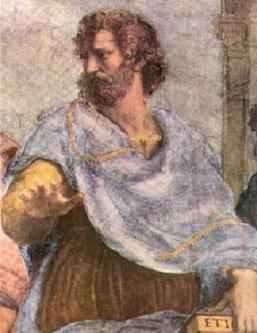
\includegraphics[width=0.44\textwidth]{aristotle.jpg}
\end{wrapfigure}

\subsection{Ethica Nicomachea}

Aristoteles was een oude Griekse filosoof en wetenschapper \cite{aristotle}. 
Aristoteles geloofde dat deugd essentieel was om het uiteindelijke doel te bereiken: geluk.\\ 
\noindent Als een deel van de filosofie\"en beschreven in zijn werken over Ethica Nicomachea, werd een idee gevormd onder de naam \textit{"golden mean"}, die een wereld van overmaat en tekort beschreef. Deze filosofie beschreef de kwaden van de wereld - of opposities tegen de groei van het leven - als een overmaat of een tekort. De gulden middenweg wordt omschreven als de eigenschap om geen overmaat of tekort te hebben, maar eerder een 'gulden middenweg' tussen de twee uitersten.

\pagebreak
\subsection{Kingdom of Ends}

\begin{wrapfigure}{l}{0.44\textwidth}
    \centering
    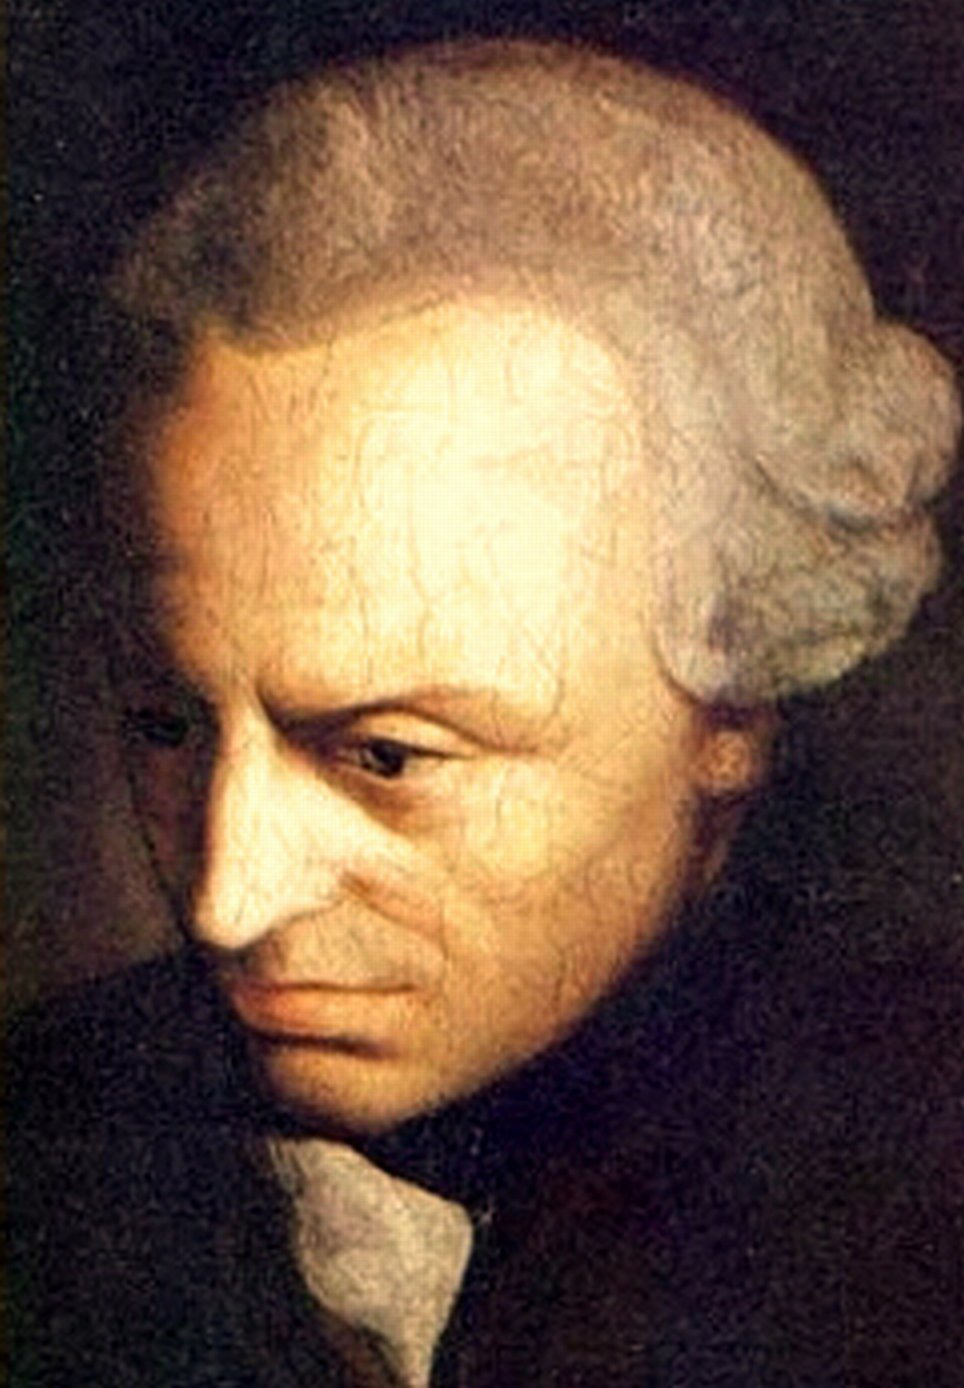
\includegraphics[width=0.44\textwidth]{kant.jpg}
\end{wrapfigure}

Immanuel Kant werd geboren voor zijn tijd op 22 april 1724 in Berlijn, Duitsland \cite{kant}. Hij had vele filosofie\"en die nog steeds worden bestudeerd tot op de dag van vandaag. Een van zijn meer opmerkelijke werken werd het \textit{Kingdom of Ends}. genoemd. Hij beschrijft een hypothetisch bestaan ​​waarin individuen volledig rationeel handelen, en met reden. Hij definieert deze mensen als degenen die in staat zijn tot correct gedrag. Hij stelde voor dat als degenen die in staat waren om te leven onder een gemeenschappelijke wet van wetten die van het grootste belang en de noodzaak waren, dat een meer harmonieuze en \textit{morele} samenleving zich zou kunnen vormen als een \textit{Kingdom of Ends}.\\

\noindent Deze gemeenschappelijke wetten kunnen worden beschouwd als referentiepunten voor de waarde van acties in een Kingdom of Ends, waar de correlatie met universele wetgeving de grootste waarde heeft voor die van Kingdom of Ends. Zijn tweede formulering toonde aan dat individuen die in overeenstemming met het principe leven om medemensen als een doel op zichzelf te behandelen, in staat waren tot grotere deugd, en daarom, vreugde. Dit beschrijft een idee en een filosofie van handelen in overeenstemming en harmonie mensen als een koninkrijk van doelen, in plaats van dat elk individu op zoek is naar elkaar als middel voor hun eigen doeleinden.

\bigskip
\textit{"People can only belong to the Kingdom of Ends when they become subject to these universal laws. Such rational beings must regard themselves simultaneously as sovereign when making laws, and as subject when obeying them. Morality,  therefore, is acting out of reverence for all universal laws which make the Kingdom of Ends  possible. In a true Kingdom of Ends, acting virtuously will be rewarded with happiness."} \footnote{Overgenomen van \url{https://en.wikipedia.org/wiki/Kingdom_of_Ends}}

\subsection{The Tao}

In het oude China was de bewaarder van de Imperiale Bibliotheek, Lao Tzu, beroemd om zijn wijsheid. Toen hij de toenemende corruptie van de regering zag, vertrok hij naar het platteland. Onderweg vroeg de bewaker bij de stadspoorten Lao Tzuto om de essentie van zijn begrip uit te schrijven om toekomstige generaties ten goede te komen. Lao Tzu schreef de Tao Te Ching, vertrok, en er werd nooit meer iets van hem gehoord \cite{tao_introduction}.

\medskip
\begin{center}
\textbf{\cite{tao_chapter1} Hoofdstuk 1 van de Tao Te Ching:}
\end{center}

\begin{wrapfigure}[20]{r}{0.25\textwidth}
    \centering
    \vspace{-45pt}
    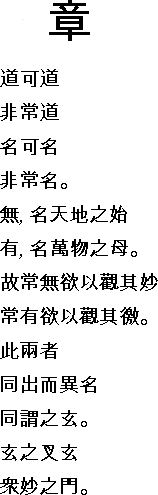
\includegraphics[width=0.30\textwidth]{tao.png}
\end{wrapfigure}

\noindent
\vspace{-10pt}
\begin{flushright}
De "Tao" is te groot om te worden beschreven door de naam "Tao". Als het zo eenvoudig genoemd zou kunnen worden, zou het niet de eeuwige Tao zijn.\vspace{10pt}\linebreak
Hemel en Aarde begonnen met de naamloze (Tao), maar de massa's 
dingen om ons heen werden met namen gemaakt.\vspace{10pt}\linebreak
We willen de wereld begrijpen door namen te geven aan de dingen die we zien, maar deze dingen zijn slechts de effecten van iets subtiels.\vspace{10pt}\linebreak
Wanneer we verder kijken dan de wens om namen te gebruiken, kunnen we de naamloze oorzaak van deze effecten voelen. \vspace{10pt}\linebreak
De oorzaak en de effecten zijn aspecten van hetzelfde, \'e\'en ding. Ze zijn zowel mysterieus als diepzinnig.\vspace{20pt}\linebreak
Op hun meest mysterieuze en diepzinnige punt ligt de \textit{"Poort van de Grote Waarheid"}.
\end{flushright}

\epigraph{Mensen moeten in de eerste rechtvaardige principes hebben en dan zullen ze niet nalaten om deugdzame daden te verrichten.}{\textit{\footnotesize{Martin Luther}}}

\section{Principes}

Principes zijn de verlengstukken van filosofie\"en die gedachten raamwerken opzetten en fungeren als richtlijnen voor goed gedrag tussen onszelf en anderen.

\subsection{Individueel}

\begin{enumerate}
\item \textbf{Evalueer} als een middel tot grotere \textbf{kennis}
\item \textbf{Geluk} als gevolg van \textbf{deugd}
\item \textbf{Respect} als resultaat van \textbf{diepgang}
\item \textbf{Vrijheid} als de meest ware \textbf{uitdrukking}
\end{enumerate}

\subsection{Collectief}

\begin{enumerate}
\item \textbf{Doel} met ontvankelijkheid, \textbf{Eerlijk} in Communicatie
\item \textbf{Respectvol} in gedrag, \textbf{Begrip} in Conflict
\item \textbf{Eer} aan een gesproken Woord, \textbf{Harmonie} met Actie
\end{enumerate}

\section{Hoe we verandering maken}

De cellen van ons lichaam werken samen om de capaciteit voor het leven te bieden. Op dezelfde manier kunnen we de cellen van onze planeet met elk individu vergelijken. Als we de voordelen van samenwerking begrijpen, kunnen uitdagingen grondig en snel worden opgelost zonder onnodige problemen. Dit is hoe we verandering maken; samenwerken om haalbare oplossingen te bieden voor uitdagingen. Dit is de meest effici\"ente en effectieve manier om verandering in de richting van onze voorkeuren te sturen.\\

\noindent De gemeenschap is de basis van een economie. Een economie is alleen zo sterk als de basis. Wanneer mensen het vertrouwen in een economie verliezen, zal de basis van de economie instorten en zal de waarde van het systeem dalen. De Nexus community is reeds erg veerkrachtig tegen de stress van de markten. De community is een positieve aaneenhang van een groep mensen over de hele wereld die allemaal streven naar dezelfde doelen als transparantie, welvaart en vrijheid.\\ 

\noindent Nexus wil een sterke community opbouwen op basis van een spaarcultuur en liefdadigheid. De spaarcultuur is al lang verloren gegaan, maar het is het beste verzekeringsbeleid voor onzekere tijden die mogelijk in het verschiet liggen. Dit helpt de gemeenschap zich af te dekken tegen risicovolle en volatiele markten. Het idee is dat je communitylid je buurman is. Als je buurman het goed doet, zal je lokale economie ook gedijen. 

\section{Lijst met bijdragers}

\begingroup
\parindent 0pt
\parskip  8pt

\begin{enumerate}
\item 
\printcontributor{Cantrell}

\item
\printcontributor{Reeg}

\item
\printcontributor{Gmyrek}

\item
\printcontributor{pSmith}

\item
\printcontributor{kSmith}

\item
\printcontributor{jSmith}

\item
\printcontributor{Mara}

\item
\printcontributor{gBogaerts}

\item
\printcontributor{Nexus}
\end{enumerate}

\endgroup

\pagebreak
\begin{thebibliography}{7}

\bibitem{bitcoin}
Bitcoin: A Peer-to-Peer Electronic Cash System \url{https://bitcoin.org/bitcoin.pdf}

\bibitem{hyperinflation}
Wat zijn enkele historische voorbeelden van hyperinflatie? Investopedia.
\url{http://www.investopedia.com/ask/answers/061515/what-are-some-historic-examples-hyperinflation.asp}

\bibitem{cbc}
William F. Ehrsam, Carl H. W. Meyer, John L. Smith, Walter L. Tuchman, "Message verification and transmission error detection by block chaining", US Patent 4074066, 1976 \url{https://en.wikipedia.org/wiki/Block_cipher_mode_of_operation}

\bibitem{meshnetworks}
Mesh networking. Wikipedia.
\url{https://en.wikipedia.org/wiki/Mesh_networking}

\bibitem{caching}
Uitleg over wat Cache of tijdelijk geheugen is
\url{https://nl.wikipedia.org/wiki/Cache_(tijdelijk_geheugen)}

\bibitem{githubnexusreleases}
Nexus releases on GitHub.com
\url{https://github.com/Nexusoft/Nexus/releases}

\bibitem{skminer}
SKMiner
\url{https://github.com/BitSlapper/SKMiner}

\bibitem{wolfniro}
Wolf Niro Miner
\url{https://github.com/OhGodAPet/Wolf-Niro-Miner}

\bibitem{wikiclockdrift}
Clock Drift. Wikipedia.
\url{https://en.wikipedia.org/wiki/Clock_drift}

\bibitem{nexusearth}
NexusEarth.com
\url{http://nexusearth.com/}

\bibitem{wikihash}
Cryptographic hash function. (2016, December 1). Wikipedia, The Free Encyclopedia. Retrieved 01:37, May 18, 2017 from \url{https://simple.wikipedia.org/w/index.php?title=Cryptographic_hash_function&oldid=5540578.}

\bibitem{peercoin}
King, S.; Nadal, S. (August 12, 2012). "PPCoin: Peer-to-peer crypto-currency with proof-of-stake" (PDF). peercoin.net. Retrieved 2013-12-23. \url{https://peercoin.net/assets/paper/peercoin-paper.pdf}

\bibitem{sect571r1} 
SEC 2: Recommended Elliptic Curve Domain Parameters, Daniel R. L. Brown (dbrown@certicom.com), Version 2.0, Section 3.7.2. 2010. Retrieved Jan 27, 2017 \url{http://www.secg.org/sec2-v2.pdf}

\bibitem{secp256k1}
secp256k1. Bitcoin Wiki.
\url{https://en.bitcoin.it/wiki/Secp256k1}

\bibitem{NIST_POST_QUANTUM}
Submission Requirements for Post Quantum Cryptography
\url{https://csrc.nist.gov/csrc/media/projects/post-quantum-cryptography/documents/call-for-proposals-final-dec-2016.pdf}
 
\bibitem{sha256bitcoin} 
Block hashing algorithm, Bitcoin Wiki \url{https://en.bitcoin.it/wiki/Block_hashing_algorithm}

\bibitem{wikisha2}
SHA-2. Wikipedia.
\url{https://en.wikipedia.org/wiki/SHA-2}

\bibitem{skeinpaper}
The Skein Hash Function Family. Version 1.3 — 1 Oct 2010.
\url{http://www.skein-hash.info/sites/default/files/skein1.3.pdf}

\bibitem{sha3announce} 
NIST Releases SHA-3 Cryptographic Hash Standard \url{https://www.nist.gov/news-events/news/2015/08/nist-releases-sha-3-cryptographic-hash-standard}

\bibitem{hashcash}
Hashcash - A Denial-of-Service Countermeasure. Adam Back. 2002. \url{http://www.hashcash.org/hashcash.pdf}

\bibitem{googlesha1}
Google Security Blog: Announcing the First SHA1 Collison. Feb 23, 2017.
\url{https://security.googleblog.com/2017/02/announcing-first-sha1-collision.html}

\bibitem{nistcompetitionend}
NIST: SHA-3 Winner, October 2nd, 2010
\url{http://csrc.nist.gov/groups/ST/hash/sha-3/winner_sha-3.html}

\bibitem{nobelfeynman}
The Nobel Prize in Physics 1965 was awarded jointly to Sin-Itiro Tomonaga, Julian Schwinger and Richard P. Feynman "for their fundamental work in quantum electrodynamics, with deep-ploughing consequences for the physics of elementary particles"
\url{http://www.nobelprize.org/nobel_prizes/physics/laureates/1965/}

\bibitem{grover2qubits}

Nature: FIGURE 4. Implementation of Grover's search algorithm, July 9th, 2009
\url{http://www.nature.com/nature/journal/v460/n7252/fig_tab/nature08121_F4.html}

\bibitem{groversalgorithm}

Estimating Cost of generic quantum pre-image attacks, October 13th, 2016
\url{https://arxiv.org/pdf/1603.09383.pdf}

\bibitem{cdhalving}
Will Bitcoin's Block Rewards Halving Bring Crisis or Consistency? CoinDesk.
\url{http://www.coindesk.com/crisis-halving-bitcoin-mining/ip}

\bibitem{quantumattacks}

Quantum Attacks on Public Key Cryptosystems, Song Y. Yan 2013

\url{http://www.springer.com/us/book/9781441977212}

\bibitem{bitcorepkh}
bitcore-lib docs. Script section.
\url{https://github.com/bitpay/bitcore-lib/blob/master/docs/script.md}

\bibitem{goldenmean}
Golden Mean.
\url{http://www.anus.com/zine/articles/draugdur/golden_mean/}

\bibitem{n_ethics}
Nicomachean Ethics. Wikipedia.
\url{https://en.wikipedia.org/wiki/Nicomachean_Ethics}

\bibitem{aynrand}
Objectivism (Ayn Rand). Wikipedia.
\url{https://en.wikipedia.org/wiki/Objectivism_(Ayn_Rand)}

\bibitem{kingdomofends}
Kingdom of Ends. Wikipedia.
\url{https://en.wikipedia.org/wiki/Kingdom_of_Ends}

\bibitem{aristotle}
Aristotole. Wikipedia.
\url{https://en.wikipedia.org/wiki/Aristotle}

\bibitem{kant}
Immanuel Kant. Wikipedia.
\url{https://en.wikipedia.org/wiki/Immanuel_Kant}

\bibitem{tao_introduction}
TheTao.info
\url{http://www.thetao.info/index.htm}

\bibitem{tao_chapter1}
TheTao.info Chaper 1.
\url{http://www.thetao.info/english/page1.htm}

\bibitem{tragedycommons}
Tragedy of the Commons. Investopedia.
\url{http://www.investopedia.com/terms/t/tragedy-of-the-commons.asp}

\bibitem{primesolominer}
Nexus Prime Solo Miner Source Code, Github.com
\url{https://github.com/Nexusoft/PrimeSoloMiner}

\bibitem{nxsprimecom}
NXSPrime.com
\url{http://nxsprime.com}

\bibitem{wikiprobable}
Probable prime. Wikipedia.
\url{https://en.wikipedia.org/wiki/Probable_prime}

\bibitem{wikifermat}
Fermat primality test. Wikipedia.
\url{https://en.wikipedia.org/wiki/Fermat_primality_test}

\bibitem{findingprimeclusterspaper}
Finding Clusters of Primes, I, Jorg Waldvogel and Peter Leikauf, January 2003.
\url{http://www.sam.math.ethz.ch/~waldvoge/Projects/clprimes03.pdf}

\bibitem{wolframprimecluster}
Prime Constellation - Wolfram MathWorld
\url{http://mathworld.wolfram.com/PrimeConstellation.html}

\bibitem{wikiprimecluster}
Wikipedia. Prime k-tuple: Prime Constellations
\url{https://en.wikipedia.org/wiki/Prime_k-tuple#Prime_constellations}

\bibitem{physicsmathprime}
Quantum Magazine: Physicists Attack Math's \$1,000,000 Question.
\url{https://www.quantamagazine.org/quantum-physicists-attack-the-riemann-hypothesis-20170404/}

\bibitem{shorarxiv}
Polynomial-Time Algorithms for Prime Factorization and Discrete Logarithms on a Quantum Computer. Peter W. Shor (AT\&T Research).
\url{http://arxiv.org/abs/quant-ph/9508027}

\bibitem{prooszalka}
J. Proos, C. Zalka, Shor's discrete logarithm quantum algorithm for elliptic curves. Quant. Inf. Comput. 3(4), 317-344 (2003).
\url{https://arxiv.org/abs/quant-ph/0301141}

\bibitem{kayezalka}
Optimized quantum implementation of elliptic curve arithmetic over binary fields. Phillip Kaye, Christof Zalka. 2004.
\url{https://arxiv.org/abs/quant-ph/0407095}

\bibitem{registersha3}
SHA3-256 is quantum-proof, should last BEELLIONS of years, say boffins. The Register.
\url{http://www.theregister.co.uk/2016/10/18/sha3256_good_for_beelions_of_years_say_boffins/}

\bibitem{cryptosha3}
Estimating the cost of generic quantum pre-image attacks on SHA-2 and SHA-3
\url{http://eprint.iacr.org/2016/992}

\bibitem{sigleak}
"Ooh Aah... Just a Little Bit" : A small amount of side channel can go a long way. N. Benger, J. van der Pol, Nigel P. Smart and Y. Yarom.
\url{http://eprint.iacr.org/2014/161}

\bibitem{sidechannel}
Recovering OpenSSL ECDSA Nonces Using the FLUSH+RELOAD Cache Side-channel Attack. Yuval Yarom. Naomi Benger. February 24, 2014.
\url{https://eprint.iacr.org/2014/140.pdf}

\bibitem{weusesand}
The Amazing Math of Bitcoin Private Keys - James DeAngelo. WeUseCoins.com.
\url{https://www.weusecoins.com/amazing-math-bitcoin-private-keys/}

\bibitem{bitwiki256}
SHA-256. Bitcoin Wiki.
\url{https://en.bitcoin.it/wiki/SHA-256}

\bibitem{sha3}
SHA-3. Wikipedia.
\url{https://en.wikipedia.org/wiki/SHA-3}

\bibitem{nistgovk}
NIST Selects Winner of Secure Hash Algorithm (SHA-3) Competition. October 02, 2012. NIST.gov
\url{https://www.nist.gov/news-events/news/2012/10/nist-selects-winner-secure-hash-algorithm-sha-3-competition}

\bibitem{wikiskein}
Skein (hash function). Wikipedia.
\url{https://en.wikipedia.org/wiki/Skein_(hash_function)}

\bibitem{largebitcoin}
The Large Bitcoin Collider Is Generating Trillions of Keys and Breaking Into Wallets. Jordan Pearson. Apr 13 2017. MOTHERBOARD.
\url{https://motherboard.vice.com/en_us/article/nzpv8m/the-large-bitcoin-collider-is-generating-trillions-of-keys-and-breaking-into-wallets}

\bibitem{wikikeysize}
Key Size. Wikipedia.
\url{https://en.wikipedia.org/wiki/Key_size}

\bibitem{nsa384}
"Information Assurance". Nsa.gov. 2016-05-04. Archived on 2009-02-07. Retrieved July 2017.
\url{https://web.archive.org/web/20090207005135/http://www.nsa.gov/ia/programs/suiteb_cryptography/index.shtml}

\bibitem{bruteforce}
Cryptography/Brute force attack. Wikibooks.org. Retrived on July 2, 2017.
\url{https://en.wikibooks.org/wiki/Cryptography/Brute_force_attack}

\bibitem{p2pkh}
Bitcoin Developer Guide. P2PKH Script Validation. Bitcoin.org
\url{https://bitcoin.org/en/developer-guide#p2pkh-script-validation}

\bibitem{lovgrover}
A fast quantum mechanical algorithm for database search. Lov K. Grover (Bell Labs, Murray Hill NJ)
\url{https://arxiv.org/abs/quant-ph/9605043}

\end{thebibliography}

\end{document}
